% ****** Start of file apssamp.tex ******
%
%   This file is part of the APS files in the REVTeX 4.1 distribution.
%   Version 4.1r of REVTeX, August 2010
%
%   Copyright (c) 2009, 2010 The American Physical Society.
%
%   See the REVTeX 4 README file for restrictions and more information.
%
% TeX'ing this file requires that you have AMS-LaTeX 2.0 installed
% as well as the rest of the prerequisites for REVTeX 4.1
%
% See the REVTeX 4 README file
% It also requires running BibTeX. The commands are as follows:
%
%  1)  latex apssamp.tex
%  2)  bibtex apssamp
%  3)  latex apssamp.tex
%  4)  latex apssamp.tex
%
\documentclass[%
 reprint,
%superscriptaddress,
%groupedaddress,
%unsortedaddress,
%runinaddress,
%frontmatterverbose, 
%preprint,
%showpacs,preprintnumbers,
%nofootinbib,
%nobibnotes,
%bibnotes,
 amsmath,amssymb,
 aps,
pra,
%prb,
%rmp,
%prstab,
%prstper,
%floatfix,
]{revtex4-1}

\usepackage{physics}
\usepackage{graphicx}% Include figure files
\usepackage{dcolumn}% Align table columns on decimal point
\usepackage{bm}% bold math
\usepackage{chemformula}
%\usepackage{hyperref}% add hypertext capabilities
%\usepackage[mathlines]{lineno}% Enable numbering of text and display math
%\linenumbers\relax % Commence numbering lines

%\usepackage[showframe,%Uncomment any one of the following lines to test 
%%scale=0.7, marginratio={1:1, 2:3}, ignoreall,% default settings
%%text={7in,10in},centering,
%%margin=1.5in,
%%total={6.5in,8.75in}, top=1.2in, left=0.9in, includefoot,
%%height=10in,a5paper,hmargin={3cm,0.8in},
%]{geometry}

\usepackage{../macros/mydefs}

\begin{document}

%\preprint{APS/123-QED}

\title{Applications of \ch{MoS2} as a Two-Dimensional Material Beyond Graphene}% Force line breaks with \\
%\thanks{Term paper for PHY 7050: Winter 2015}%

\author{Kraig Andrews}%
 \email{kraig.andrews@wayne.edu}
\affiliation{%
 Wayne State University Department of Physics and Astronomy%\\
}%

%\collaboration{MUSO Collaboration}%\noaffiliation


%\collaboration{CLEO Collaboration}%\noaffiliation

\date{\today}% It is always \today, today,
             %  but any date may be explicitly specified

\begin{abstract}
An article usually includes an abstract, a concise summary of the work
covered at length in the main body of the article. 
\end{abstract}

%\pacs{Valid PACS appear here}% PACS, the Physics and Astronomy
                             % Classification Scheme.
%\keywords{Suggested keywords}%Use showkeys class option if keyword
                              %display desired
\maketitle

%\tableofcontents

\section{\label{sec:introduction} Introduction}

\section{\label{sec:graphene_properties} Graphene as a New Two-Dimensional Material}
\subsection{\label{subsec:discovery} The Discovery of Graphene}
By the end of the last century microelectronics had revolutionized the world, the majority which are silicon-based devices. Today, millions of these silicon-based devices are used in many common electronic devices and have become unavoidable throughout everyday life. Though the first field-effect device was patented in 1925, it was not until 1960 that the first metal-oxide semiconductor field effect transistor was demonstrated \cite{Lilienfeld1925, Atalla1960, Schulz1999}. A decade after the first device, devices were being made with several thousand components on a single chip. From there the progress increased at a rapid rate, a process now known as Moore's law, predicting that for each new generation of memory chip and microprocessor unit, the device size would be reduced by 33\%, the chip size would be increased by 50\%, and the number of components on a chip would quadruple every three years \cite{Schulz1999, Moore1965}. This proven to be true, and up until recently had shown no signs of stopping. Many times the material limitations were overcome by advances in technology that were seemingly insurmountable and effectively had placed a cap on Moore's law, which ultimately led to new techniques and even more pristine silicon-based materials. However, the limit to oxide thickness has finally placed a maximum on the growth of the silicon-based semiconductor device industy \cite{Schulz1999}. This impending limit caused many to look for solutions that involved the use of \ch{SiO2} devices and also alternatives to silicon. The result of the latter has given way to a breadth of literature and research that was unforseen a decade before. The search for alternatives to silicon resulted in research into many new, nontraditional materials. Several notable examples are organic conductors and carbon nanotubes \cite{Mascaro2001, Baughman2002}. Arguably one of the most interesting nontraditional materials to come out of such research was graphene. 

In 1985, with the discovery of fullerenes the amount of known carbon allotropes increased \cite{krotoFullerenes1985, nanoscaleReview2011}. Fullerenes suggested the existence of a one-dimensional form of carbon, known as carbon nanotubes, which were first demonstrated in 1991 \cite{iijimaCarbonNanotubes1991}. Despite several theoretical studies involving the use of a single layer of graphite, it was not until 2004 that the first monolayer graphene sheet was isolated \cite{novoselovEtAl2004, novoselovEtAl2005}. In the most basic sense, graphene is simply a single layer of carbon atoms densely packed into a honeycomb lattice. It is used to describe properties several carbon-based materials (graphite, fullerenes, nanotubes, etc..., see Fig.\ref{fig:sp2}) \cite{Dresselhaus2002, Brenner2002, novoselovEtAl2004}. This was significant because scientists had tried for many years to synthesize monolayers of graphite, though only succeeding in obtaining materials around 10 layers thick \cite{nanoscaleReview2011}.

\begin{figure}
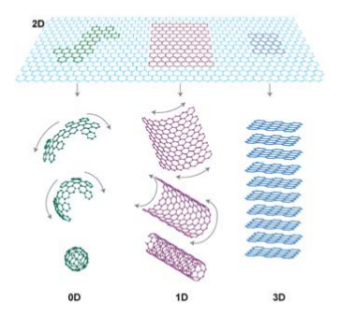
\includegraphics[height=5cm, width=5cm]{../figs/multiDimGraphene}
\caption{Graphene can be envisioned in several dimensions. 0-dimensional buckyballs, 1-dimensional nanotubes, or 3-dimensional graphite (Originally found in \cite{Novoselov2007}.)}
\label{fig:sp2}
\end{figure}

\subsection{\label{subsec:properties_graphene} Properties of Graphene}

\section{\label{sec:TMDs} Transition Metal Dichalcogenides}

\subsection{\label{subsec:mos2_properties} Properties of \ch{MoS2}}

\section{\label{sec:synthesis_methods} Synthesis Methods}

\section{\label{sec:mos2_applications} Applications of \ch{MoS2}}

\section{\label{sec:state_of_the_art} State of the Art}

\section{\label{sec:problems_and_outlook} Problems and Outlook}


\bibliographystyle{plain}
\bibliography{../bibs/refs}
\end{document}
%
% ****** End of file apssamp.tex ******

